\documentclass[a4paper]{article}

%% Language and font encodings
\usepackage[english]{babel}
\usepackage[utf8x]{inputenc}
\usepackage[T1]{fontenc}

%% Sets page size and margins
\usepackage[a4paper,top=3cm,bottom=2cm,left=3cm,right=3cm,marginparwidth=1.75cm]{geometry}

%% Useful packages
%%%%%%%%% begin snippet
%% You need to add the package "tabularx".
%% Place the snippet right after \begin{document}

% need tabularx
\usepackage{tabularx}
\usepackage{amsmath}
\usepackage{graphicx}
\usepackage[colorinlistoftodos]{todonotes}
\usepackage{paralist}
\usepackage{amssymb,amsmath,amsthm,enumitem}
\usepackage[colorlinks=true, allcolors=blue]{hyperref}
\usepackage{subcaption}
\setlength{\abovedisplayskip}{3pt}
\setlength{\belowdisplayskip}{3pt}
\usepackage[hypcap=false]{caption}

\begin{document}
\title{ Computational Intelligence, SS2018 Assignment 1}

\begin{titlepage}
       \begin{center}
             \begin{huge}
				   %% Update assignment number here
                   \textbf{Assignment 1}
             \end{huge}
       \end{center}

       \begin{center}
             \begin{large}
                   Computational Intelligence, SS2018
             \end{large}
       \end{center}

       \begin{center}
 \begin{tabularx}{\textwidth}{|>{\hsize=.33\hsize}X|>{\hsize=.33\hsize}X|>{\hsize=.33\hsize}X|} 

                   \hline
                   \multicolumn{3}{|c|}{\textbf{Team Members}} \\
                   \hline
                   STRUGER & Patrick & 01530664 \\
                   \hline
                   B\"OCK & Manfred & 01530598 \\
                   \hline
                   HAUPT & Anna & 01432018 \\
                   \hline

             \end{tabularx}
       \end{center}

\end{titlepage}

%%%%%%%%% end snippet

\newpage

\section{Linear Regression}
\subsection{Derivation of Regularized Linear Regression}
Given the design matrix $X (m~ rows, n + 1~ columns)$, output vector y (m rows) and parameter vector $\theta (n + 1 ~ rows)$, the mean squared error cost function for linear regression can be written compactly as,
\[
J(\theta)=\frac{1}{m}\left\|{X\theta-y}\right\|^2.
\]The notation $\left\|\cdot\right\| $ refers to the Euclidean norm. The optimal parameters which minimize this cost function are given by,\[
\theta^*= (X^TX)^{-1}X^Ty
\]Consider the following slightly extended, “regularized” cost function:
\[
J(\theta)=\frac{1}{m}\left\|{X\theta-y}\right\|^2 + \frac{\lambda}{m}\left\|\theta\right\|^2
\]
The additional term penalizes parameters of large magnitudes. The constant $\lambda \geq 0$ controls the influence of this penalization (low $\lambda \rightarrow$ weak regularization, high $\lambda \rightarrow $ strong regularization). Such regularized cost functions are often used for linear regression (and other learning models) instead of (1) because regularization drastically reduces the effects of over-fitting that occur when the number of features is large.

\subsubsection{Answer the following questions:}
\begin{itemize}
\item Preliminary questions
\begin{compactenum}[-]
\item \textbf{why is the design matrix $X$ containing $n + 1 $ columns and not just $n$?} \\
\newline
The first column of the design matrix consists of ones for \textit{convenience} which allow estimation of y-intersept. The following columns contain the x-values associated with their related values of y. \\

\item \textbf{considering the function $J(\theta)$ as a function of all the variables $\theta_0,\theta_1 ... $ , what is the definition of the gradient ~$\frac{\partial J(\theta)}{\partial\theta}$? This gradient is actually a vector, what is its dimension?} \\

\[
J(\theta) = \frac{1}{m} \lVert X\theta - y \rVert^2 + \frac{\lambda}{m} * \lVert \theta \rVert^2
\]

\textbf{Gradient definition}

\begin{align}
\frac{\partial J(\theta)}{\partial\theta} = \frac{2}{m} * \frac{\partial(X\theta - y)^T ~ (X\theta -y)}{\partial \theta} + \frac{2 \lambda}{m} * \frac{\partial(\theta)^T \theta}{\partial \theta} \\
\Rightarrow \frac{2}{m} * (X\theta - y)^T * \frac{\partial(X\theta - y)}{\partial \theta} + \frac{2 \lambda}{m} * (\theta)^T * \frac{\partial(\theta)}{\partial \theta} \\
\Rightarrow \frac{2}{m} * (X\theta - y)^T * X + \frac{2\lambda}{m} * (\theta)^T
\end{align}

The gradient vector is formed with the partial derivatives. The dimension of the gradient is the amount of columns in the given matrix X (if $X = m~*~n$ then gradient of the form $1~*~n$).\\

\item \textbf{What is the definition of the Jacobian matrix and what is the difference between the gradient and
the Jacobian matrix?} \\
\newline
The Jacobian Matrix is a $m~*~n$ matrix of a differentiable function $f: \mathbb{R}^n \rightarrow \mathbb{R}^m$ formed with the partial derivatives. The gradient matrix $1~*~n$ is used for functions of the form $f: \mathbb{R}^n \rightarrow \mathbb{R}$. \\

\newpage

\item \textbf{the hypothesis $X\theta$ generates predictions of the output vector $y$, each coordinate of the vector corresponds to a different data point. What is the dimension of the vector $X\theta$? We also use
the notation $\frac{\partial X(\theta)}{\partial\theta}$ to define the Jacobian matrix. What is the dimension of the Jacobian matrix$\frac{\partial X(\theta)}{\partial\theta}$? In this particular case, what is $\frac{\partial X(\theta)}{\partial\theta}$ equal to?} \\
\newline
The vector $X\theta$ has the same dimension as the provided output vector  ($m * 1$) which refers to the number of training examples.\\
The dimension of the  Jacobian matrix$\frac{\partial X(\theta)}{\partial\theta}$ is m *(n+1) and this is equal to the design matrix X.


\end{compactenum}

\item{Using the following hints, show that the optimal parameters which minimize the regularized linear regression cost (3) are given by, $\theta^{*}=(X^{T}X+\lambda I)^{-1}X^{T}y$, where $I$ denotes the identity matrix of dimension $(n+1) \times (n+1)$.}

\begin{align}
\frac{\partial J(\theta)}{\partial \theta} = 0 \\
\Rightarrow \frac{2}{m} * (X\theta - y)^T * X * \frac{2\lambda}{m} * (\theta)^T = 0 \\
\Rightarrow \frac{2}{m} ((X\theta - y)^T * X + \lambda * (\theta)^T)) = 0 \\
\Rightarrow ((X\theta - y)^T * X + \lambda * (\theta)^T)) = 0 \\
\Rightarrow (X\theta - y)^T * X = -\lambda(\theta)^T \\
\Rightarrow (X^T\theta^T - y^T) * X = -\lambda(\theta)^T \\
\Rightarrow (X^T\theta^TX - y^TX) = -\lambda(\theta)^T \\
\Rightarrow (X^T\theta^TX + \lambda(\theta)^T) = y^TX \\
\Rightarrow \theta^T(X^TX + \lambda) = y^TX \\
\Rightarrow \theta^T(X^TX + \lambda)(X^TX + \lambda)^{-1} = (X^TX + \lambda)^{-1} y^TX \\
\Rightarrow \theta^T = (X^TX + \lambda)^{-1} y^TX \\
\Rightarrow \theta^* = (X^TX + \lambda I)^{-1} * yX^T \\
\end{align}

\item{(Optional) In practice the matrix $X^{T} X$ might not be invertible. Using the spectral theorem (eigenvalue
decomposition of symmetric matrices), what can we say about the eigenvalues of $X^{T} X$ ? Explain why
the matrix $X^{T} X + \lambda I$ is invertible for any small positive $\lambda$.}
\end{itemize}

\newpage

\subsection{Linear Regression with polynomial features }
Your task is to fit polynomials of different degrees to the training data, and to identify the degree which gives
the best predictions on the validation set (performing simple model selection). The features that should be
used for linear regression are ($x$ corresponds to the scalar input, and $n$ is the polynomial degree)
\[\phi_0 = 1, \phi_1 = x, \phi_2 = x^2, . . . , \phi_n = x^n\]

\begin{itemize} 
\item \textbf{Plot your results for each of the following polynomial degrees: 1, 2, 5, 20.}\\
\begin{minipage}[b]{0.4\textwidth}
  \vspace{10pt}
  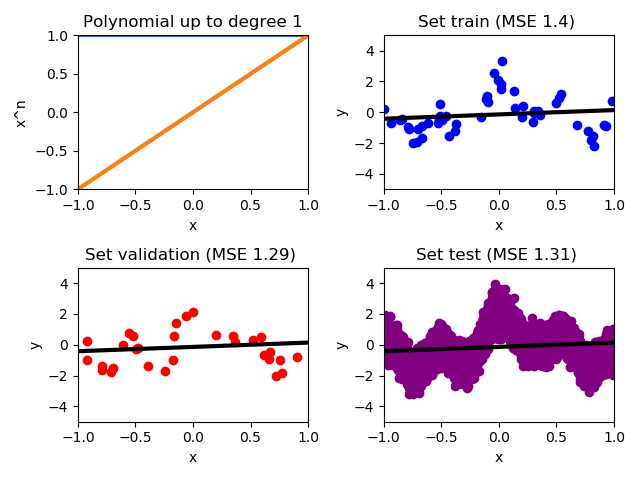
\includegraphics[scale=0.35]{plots/plot_poly_degree1.png}
 \captionsetup{justification=centering}
  \captionof{figure}{Plot with polynomial degree of 1}
  \label{plot_poly_degree1}
\end{minipage}
\hfill
\begin{minipage}[b]{0.4\textwidth}
  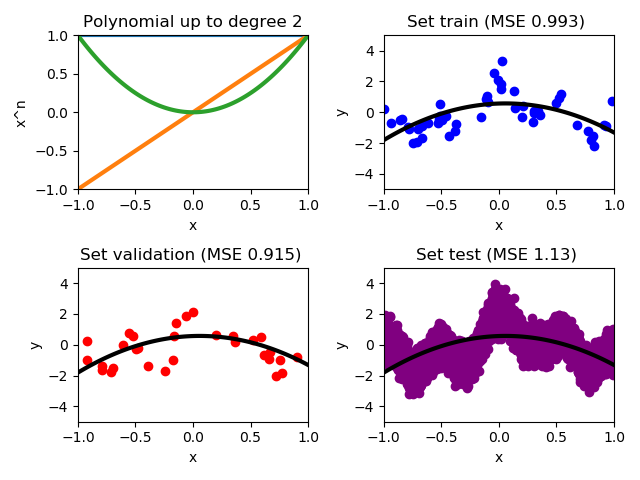
\includegraphics[scale=0.35]{plots/plot_poly_degree2.png}
 \captionsetup{justification=centering}
  \captionof{figure}{Plot with a polynomial degree of 2}
  \label{plot_poly_degree2}
\end{minipage}
\begin{minipage}[b]{0.4\textwidth}
  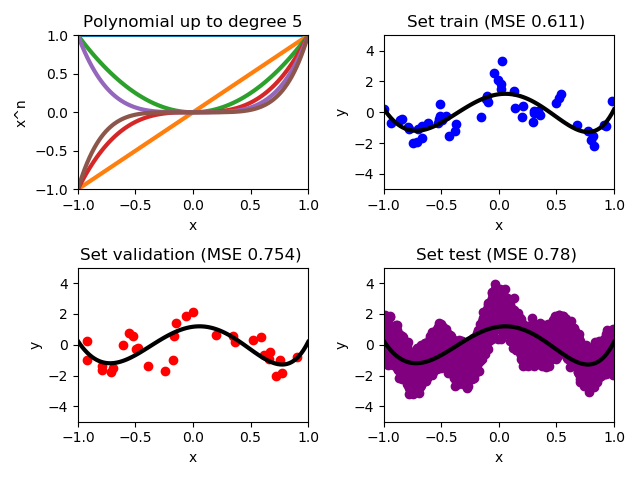
\includegraphics[scale=0.35]{plots/plot_poly_degree5.png}
 \captionsetup{justification=centering}
  \captionof{figure}{Plot with a polynomial degree of 5}
  \label{plot_poly_degree5}
\end{minipage}
\hfill
\begin{minipage}[b]{0.4\textwidth}
  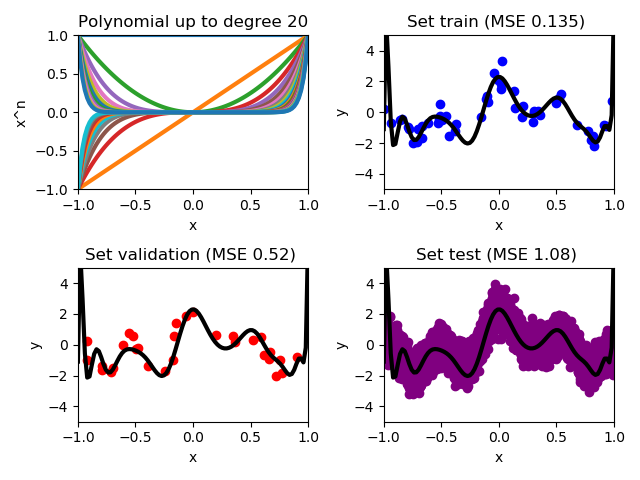
\includegraphics[scale=0.35]{plots/plot_poly_degree20.png}
 \captionsetup{justification=centering}
  \captionof{figure}{Plot with a polynomial degree of 20}
  \label{plot_poly_degree20}
\end{minipage}

\newpage

\item \textbf{Report which degree $\in  \{1, . . . , 30\}$ gives the lowest training error. Plot the results for that degree. Report the test error.} \\
\textcolor{blue}{ The lowest Trainings Error produced the plot with a degree of 30 it was only 0.1257193081096509. The related Testing Error was 14.888677131456754.}
\begin{figure}[ht]
    \centering
  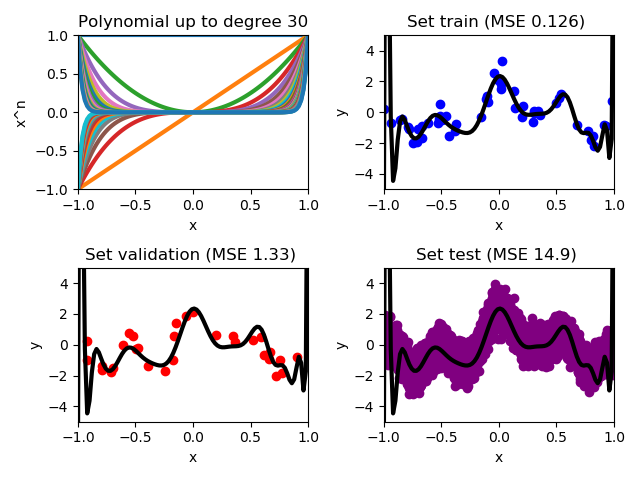
\includegraphics[scale=0.50]{plots/plot_poly_degree30.png}
 \captionsetup{justification=centering}
  \caption{Lowest Trainings Error}
    \label{plot_poly_degree30_lowest_trainings_error}
  \end{figure}
\item \textbf{Report which degree $\in  \{1, . . . , 30\}$ gives the lowest validation error. Plot the results for that degree. Report the test error.} \\
\textcolor{blue}{ The lowest Validation Error produced the plot with a degree of 13 it was only 0.30522863334865147. The related Testing Error was 0.38370160426301475.}
\begin{figure}[ht]
    \centering
  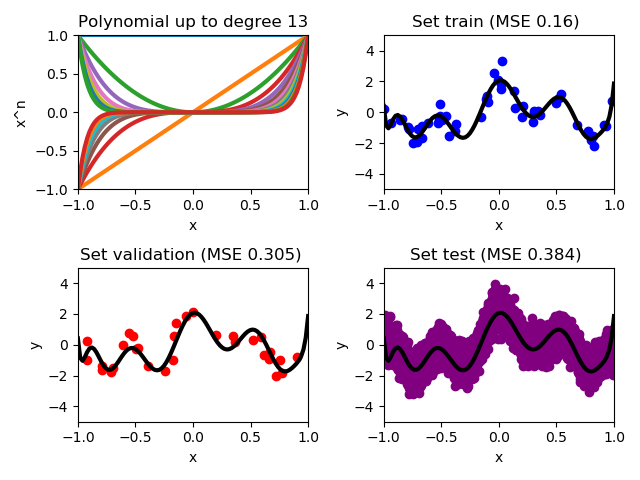
\includegraphics[scale=0.50]{plots/plot_poly_degree13.png}
 \captionsetup{justification=centering}
  \caption{Lowest Validation Error}
    \label{plot_poly_degree13_lowest_validation_error}
  \end{figure}
  
\newpage
\item \textbf{Plot training, validation and testing errors as a function of the polynomial degree.} \\
\begin{figure}[ht]
    \centering
 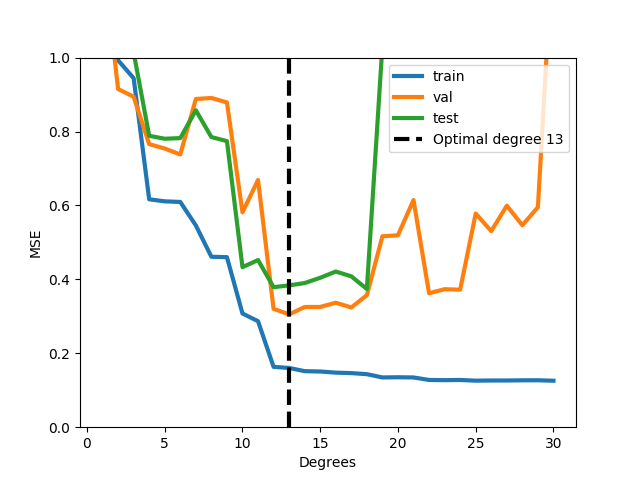
\includegraphics[scale=0.50]{plots/plot_poly_function_of_polynomial_degree.png}
 \captionsetup{justification=centering}
  \caption{Training, Validation \& Testing Errors as functions of the polynomial degree}
    \label{plot_poly_function_of_polynomial_degree}
  \end{figure}
\item \textbf{Discuss your findings in your own words using the concept of over-fitting. Why is it important to use a validation set?} \\
\textcolor{blue}{ We found out that at first the error for Trainings, Testing \& Validation sets is reduced more or less equally but at a certain degree the errors in the training set still decreases but only minimally,  whereas the errors in the Testing \& Validation sets drastically deteriorated that phenomenon is called \textit{over-fitting}
It is important to use a validation set to get an ideal mean value for the used degree so that the error for all data is kept as small as possible to be precise to find the hypothesis which produces the best results .
} 
\end{itemize}

\newpage

\subsection{Linear Regression with radial basis functions}
Using the same data set, your task is to fit hypotheses with different numbers of radial basis functions to the
training data, and to perform model selection. Let l be the number of RBFs. For a given $l$, the RBF centers
should be chosen to uniformly span the whole input range $[−1, 1]$. The width of the basis functions should
be set to $\sigma = 2/l$, i.e. with a higher $l$, the RBFs should be narrower (implementing a finer resolution). The
features used for linear regression should be ($x$ corresponds to the scalar input and $c_j$ is the center of RBF
$j$)
\[
\phi_0 = 1, \phi_1 = e^{\frac{-(x-c_1)^2}{2\sigma^2}}, ... , \phi_l = e^{\frac{-(x-c_l)^2}{2\sigma^2}}
\]

\vspace{10pt}
\begin{itemize}
\item \textbf{Plot your results for each of the following degrees: 1, 2, 5, 20.}\\

\begin{minipage}[b]{0.4\textwidth}
  \vspace{10pt}
  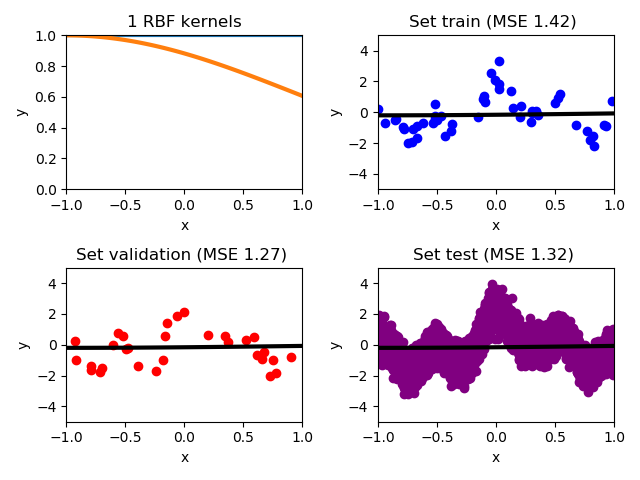
\includegraphics[scale=0.35]{plots/plot_rbf_degree1.png}
 \captionsetup{justification=centering}
  \captionof{figure}{Radial Basis Function with a degree of 1}
  \label{plot_rbf_degree1}
\end{minipage}
\hfill
\begin{minipage}[b]{0.4\textwidth}
  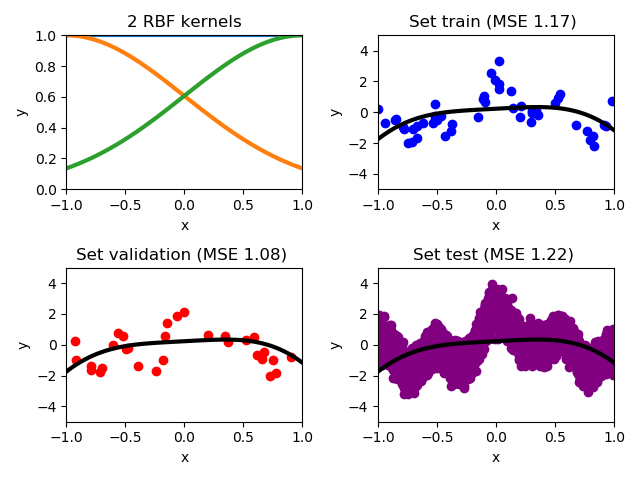
\includegraphics[scale=0.35]{plots/plot_rbf_degree2.png}
 \captionsetup{justification=centering}
  \captionof{figure}{Radal Basis Function with a degree of 2}
  \label{plot_rbf_degree2}
\end{minipage}

\begin{minipage}[b]{0.4\textwidth}
  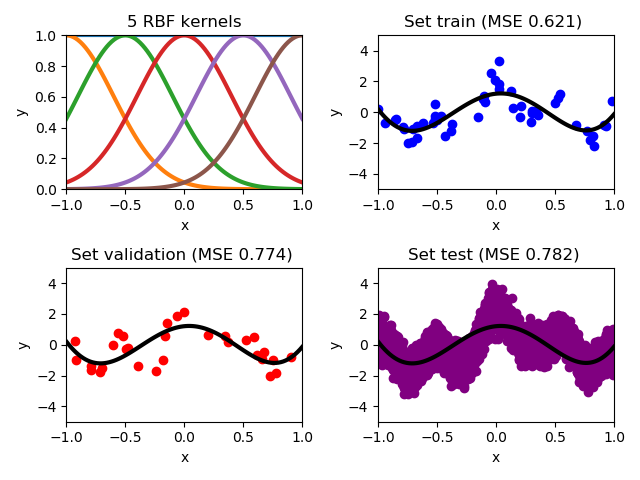
\includegraphics[scale=0.35]{plots/plot_rbf_degree5.png}
 \captionsetup{justification=centering} 
  \captionof{figure}{Radial Basis Function with a degree of 5}
  \label{plot_rbf_degree5}
\end{minipage}
\hfill
\begin{minipage}[b]{0.4\textwidth}
  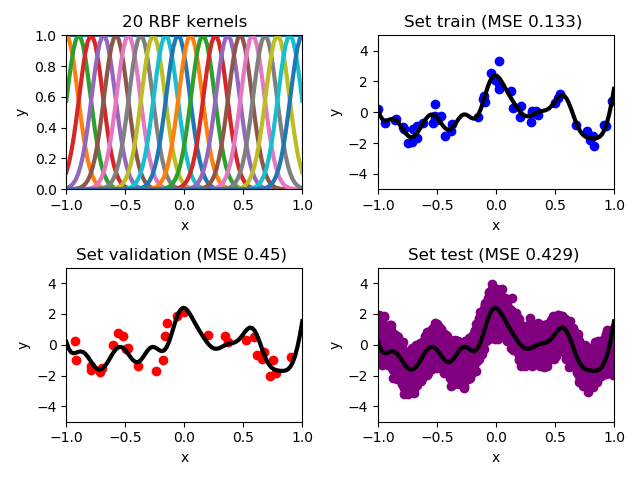
\includegraphics[scale=0.35]{plots/plot_rbf_degree20.png}
 \captionsetup{justification=centering}
  \captionof{figure}{Radial Basis Function with a degree of 20}
  \label{plot_rbf_degree20}
\end{minipage}

\newpage

\item \textbf{Report which number of RBFs $∈ \{1, . . . , 40\} $gives the lowest training error. Plot the results for that degree. Report the test error.}\\
\textcolor{blue}{The lowest Trainings Error produced the plot with a degree of 40 it was only  0.054452916301053075. The related Testing Error was 181.6718279531847.}
\begin{figure}[ht]
    \centering
  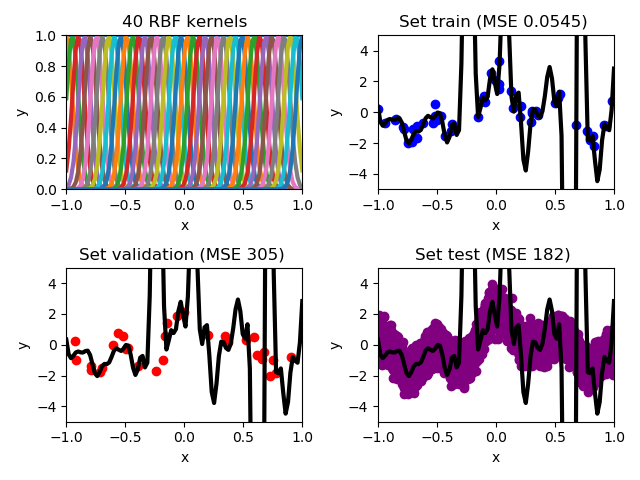
\includegraphics[scale=0.50]{plots/plot_rbf_degree40.png}
 \captionsetup{justification=centering}
  \caption{Lowest RBF Training Error}
\label{plot_rbf_degree13_lowest_validation_error}
  \end{figure}
  
\item \textbf{Report which number of RBFs $∈ \{1, . . . , 40\} $gives the lowest validation error. Plot the results for that degree. Report the test error.} \\
\textcolor{blue}{ The lowest Validation Error produced the plot with a degree of 9 it was only 0.2879598418720983. The related Testing Error was 0.33701300824089064.}
\begin{figure}[ht]
    \centering
  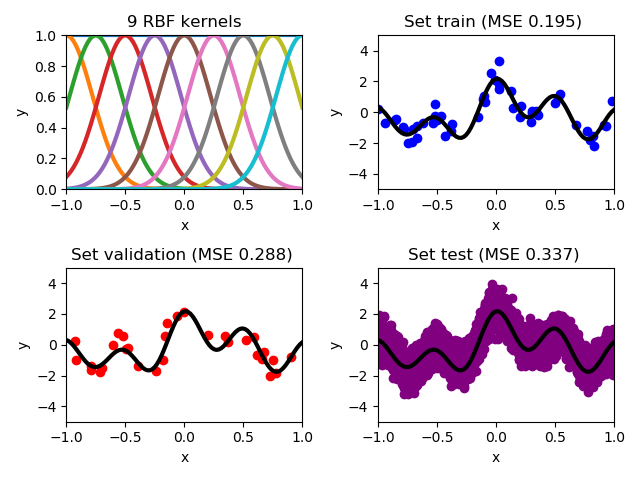
\includegraphics[scale=0.50]{plots/plot_rbf_degree9.png}
 \captionsetup{justification=centering}
  \caption{Lowest RBF Validation Error}
\label{plot_rbf_degree9_lowest_validation_error}
  \end{figure}
  
\newpage
  
\item \textbf{Plot training, validation and testing errors as a function of the degree.} \\
\begin{figure}[ht]
    \centering
  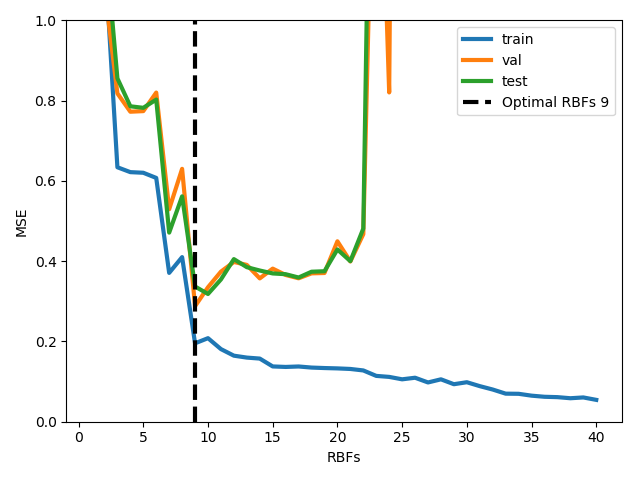
\includegraphics[scale=0.35]{plots/plot_rbf_function_of_degree.png}
 \captionsetup{justification=centering}
   \caption{Training, Validation \& Testing errors as a function of the degree}
   \label{plot_rbf_function_of_polynomial_degree}
  \end{figure}

\item \textbf{Briefly describe and discuss your findings in your own words. Is the polynomial or the RBF model better?} \\
\textcolor{blue}{ We found out that at first the error for Trainings, Testing \& Validation sets is reduced more or less equally until 9 RBFs. From this moment the errors in the training set still decreases,  whereas the errors in the Testing \& Validation sets begin to rise again. From RBF 22 the errors for the Testing \& Validation sets begin to increase immensely fast.\\
We got to the conclusion that the Radial Basis Function model superior to the Polynomial Function model because we got in almost all cases lower testing errors using the Radial Basis Function model. For example the lowest validation error had a testing error of 0,337 using the RBF model  and  a testing error of 0,384 using the Polynomial Function model.}
\end{itemize}

\newpage

\section{Logistic Regression}
\subsection{Derivation of Gradient}
The logistic regression hypothesis function is given by,
\[
h_\theta(x)=\sigma(x^T\theta) =  \sigma(\theta_0x_0+\theta_1x_1+...+\theta_nx_n)
\]with the sigmoid function $\sigma(z)=\frac{1}{1+e^{-z}}$, parameters $\sigma=(\sigma_0,\sigma_1,....,\sigma_n)^T$ , and input vector $x = (x_0,x_1,...,x_n)^T$. 
By convention the constant feature $x_0$ is fixed to $x_0 = 1$. With $x^{(i)} = (x^{(i)}_0, x^{(i)}_1,....,x^{(i)}_n)^T,x^{(i)}_0 = 1$ and $log(\cdot)$ referring to the natural logarithm, the logistic regression cost function can be written as,
\[
J(\theta)=-\frac{1}{m}\sum_{i=1}^{m}\bigg(y^{(i)} \log\Big(h_\theta(x^{(i)} )\Big)+(1-y^{(i)})\log\Big(1-h_\theta(x^{(i)} )\Big)\bigg)  
\]Derive the gradient of the cost function, i.e. show that the partial derivative of the cost function with
respect to $\theta_j$ equals
\[
\frac{\partial J (\theta)}{\partial \theta_j} = \frac{1}{m}\sum_{i=1}^{m} \Big (h_\theta(x^{(i)})-y^{(i)}\Big) \cdot x^{(i)}_j.
\] $Hint: \frac{\partial \sigma(z)}{\partial \sigma} = \sigma(z)\cdot \Big(1-\sigma(z)\Big)$

\begin{align}
\frac{\partial J (\theta)}{\partial \theta_j} = \frac{\partial}{\partial \theta_j} \bigg(-\frac{1}{m} \sum_{i=1}^{m} \bigg(y^{(i)}\log\Big(h_{\theta}(x^{(i)})\Big) + (1 + y^{(i)})\log\Big(1 - h_{\theta}(x^{(i)})\Big)\bigg)\bigg)
\end{align}
Since only the log functions contain $\theta$, we just have to do the derivation of them as follows:
\begin{align}
\Rightarrow  -\frac{1}{m} \sum_{i=1}^{m} \bigg(y^{(i)}\frac{\partial}{\partial \theta_j} \log\Big(h_{\theta}(x^{(i)})\Big) + (1 + y^{(i)}) \frac{\partial}{\partial \theta_j} \log\Big(1 - h_{\theta}(x^{(i)})\Big)\bigg) \\
\Rightarrow -\frac{1}{m} \sum_{i=1}^{m} \bigg(y^{(i)} \textcolor{blue}{\frac{1}{h\theta(x^{(i)})} \frac{\partial h\theta(x^{(i)})}{\partial \theta_j}} + (1 + y^{(i)}) \textcolor{blue}{\frac{1}{1 - h\theta(x^{(i)})} \frac{\partial (1 - h\theta(x^{(i)}))}{\partial \theta_j}}\bigg)
\end{align}
In the next step we focuse on the partial derivative $\frac{\partial(1 - h\theta(x^{(i)}))}{\partial \theta_j}$
\begin{align}
\frac{\partial(1 - h\theta(x^{(i)}))}{\partial \theta_j} = \frac{\partial}{\theta_j} \Big(1 - \frac{1}{1 + e^{-x^{(i}\theta^{(i)}}} \Big) * (x^{(i)}) = %\frac{-1 * e^{{-x^{(i)}\theta^{(i)}}} * (-x^{(i)})}{\Big(1 + e^{-x^{(i}\theta^{(i)}}\Big)^2} \\
\frac{e^{{-x^{(i)}\theta^{(i)}}} * (x^{(i)})}{\Big(1 + e^{-x^{(i}\theta^{(i)}}\Big)^2} * (x^{(i)}) = \\ \frac{\Big(-1 +1 + e^{{-x^{(i)}\theta^{(i)}}}\Big)}{\Big(1 + e^{-x^{(i}\theta^{(i)}}\Big)^2} * (x^{(i)})
= \bigg(\frac{1}{\Big(1 + e^{-x^{(i}\theta^{(i)}}\Big)} - \frac{1}{\Big(1 + e^{-x^{(i}\theta^{(i)}}\Big)^2}\bigg) * (x^{(i)})
\\ = \frac{1}{\Big(1 + e^{-x^{(i}\theta^{(i)}}\Big)} * \Big(1 - \frac{1}{\Big(1 + e^{-x^{(i}\theta^{(i)}}\Big)}\Big) * (x^{(i)}) = \Big(h\theta(x^{(i)}) * (1 - h\theta(x^{(i)}))\Big) * (x^{(i)})
\end{align}
\newpage
In the next step we compute the partial derivative $\frac{\partial h\theta(x^{(i)})}{\partial \theta_j}$ with the same scheme:

\begin{align}
\frac{\partial(h\theta(x^{(i)}))}{\partial \theta_j} = \frac{\partial}{\theta_j} \Big(\frac{1}{1 + e^{-x^{(i}\theta^{(i)}}}\Big) * (x^{(i)}) \\ 
%-\frac{-1 * e^{{-x^{(i)}\theta^{(i)}}} * (-x^{(i)})}{\Big(1 + e^{-x^{(i}\theta^{(i)}}\Big)^2}
= -\frac{e^{{-x^{(i)}\theta^{(i)}}} * (x^{(i)})}{\Big(1 + e^{-x^{(i}\theta^{(i)}}\Big)^2} * (x^{(i)}) = ... = \Big(h\theta(x^{(i)}) * (h\theta(x^{(i)}) - 1)\Big) * (x^{(i)})
\end{align}

Finally the partial derivatives are inserted in the original function

\begin{align}
\Rightarrow -\frac{1}{m} \sum_{i=1}^{m} \bigg(\frac{y^{(i)}}{h\theta(x^{(i)})} \textcolor{blue}{\Big(h\theta(x^{(i)}) * (h\theta(x^{(i)}) - 1)\Big) * (x^{(i)})} + \frac{(1 + y^{(i)})}{1 - h\theta(x^{(i)})} \textcolor{blue}{\Big(h\theta(x^{(i)}) * (1 - h\theta(x^{(i)}))\Big) * (x^{(i)})}\bigg) \\
\Rightarrow -\frac{1}{m} \sum_{i=1}^{m} \bigg(y^{(i)} \textcolor{blue}{\Big((h\theta(x^{(i)}) - 1)\Big) * (x^{(i)})} + (1 + y^{(i)}) \textcolor{blue}{\Big(h\theta(x^{(i)})\Big) * (x^{(i)})}\bigg) \\
\Rightarrow -\frac{1}{m} \sum_{i=1}^{m} \Big(y^{(i)}x^{(i)} - \textcolor{red}{y^{(i)}x^{(i)}h\theta(x^{(i)})} - x^{(i)}h\theta(x^{(i)}) + \textcolor{red}{y^{(i)}x^{(i)}h\theta(x^{(i)})}\Big) \\
\Rightarrow -\frac{1}{m} \sum_{i=1}^{m} \Big(y^{(i)}x^{(i)} - x^{(i)}h\theta(x^{(i)})\Big) \\
\Rightarrow -\frac{1}{m} \sum_{i=1}^{m} \Big(y^{(i)} - h\theta(x^{(i)}) \Big) * x^{(i)} \\
\Rightarrow \frac{1}{m} \sum_{i=1}^{m} \Big(h\theta(x^{(i)}) - y^{(i)}\Big) * x^{(i)}
\end{align}

\subsection{Logistic Regression training with gradient descent and\textit{ scipy.optimize}}
Download the associated zip file from the course website and unzip it. The file $data_logreg.json$ contains
training and test set of a binary classification problem with two input dimensions. Your task is to fit a
logistic regression classifier with polynomial features of varying degrees to the data, and to compare different
optimization techniques for this task. The optimization techniques that should be compared are gradient
descent with a constant learning rate, gradient descent with an adaptive learning rate (optional), and the
advanced optimization method implemented by the Scipy function minimize. The expansion of the input is
already implemented. The features that should be used for logistic regression are all monomials of the two
inputs $x_1$ and $x_2$ up to some degree $l$ (monomials are polynomials with only one term), i.e. all products
$(x_1)^a(x_2)^b$ with $a, b \in {Z}$ and $ a+ b \leq l$ . For example, for degree $l=3 $ the features should be,
\begin{center}
$\phi_0 = 1,$
$\phi_1=(x_1)^1, \phi_2=(x_2)^1,$
$\phi_3=(x_1)^2, \phi_4=(x_1)(x_2),\phi_5=(x_2)^2,$
$\phi_6=(x_1)^3,\phi_7=(x_1)^2(x_2)^1,\phi_8=(x_1)^1(x_2)^2,\phi_9=(x_2)^3$
\end{center}

\subsection{Gradient descent (GD)}
\begin{enumerate}
\item The function check\_gradient in toolbox.py is here to test if your gradient is well computed. Explain what it is doing.\\
\textcolor{blue}{Function check\_gradient in toolbox.py checks if the gradient \& cost functions have been computed correctly. It tries for different variations  if the gradient is with finite difference well approximated. If the gradient is well approximated a message about the success of the check is printed. On the other hand if something is not right with the cost function or the gradient an exception is raised.}
\item For degree $ l = 1$ run GD for 20 and 2000 iterations (learning rate $\eta = 1$, all three parameters initialized at zero). Report training and test errors for each iteration number and plot the decision boundaries.\\
Comment on the results and explain why the number of iterations should be neither too low nor too high.\\
\begin{minipage}[b]{0.4\textwidth}
  \vspace{10pt}
              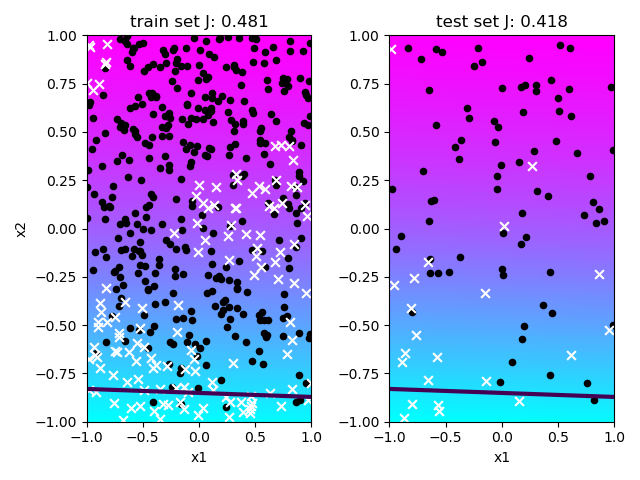
\includegraphics[scale=0.35]{plots/gradient_descent_1_1_20.png}
				\captionsetup{justification=centering}
              \captionof{figure}{GD for 20 Iterations \& Learning Rate of 1}
    \label{gradient_descent_1_1_20}
\end{minipage}
\hfill
\begin{minipage}[b]{0.4\textwidth}
              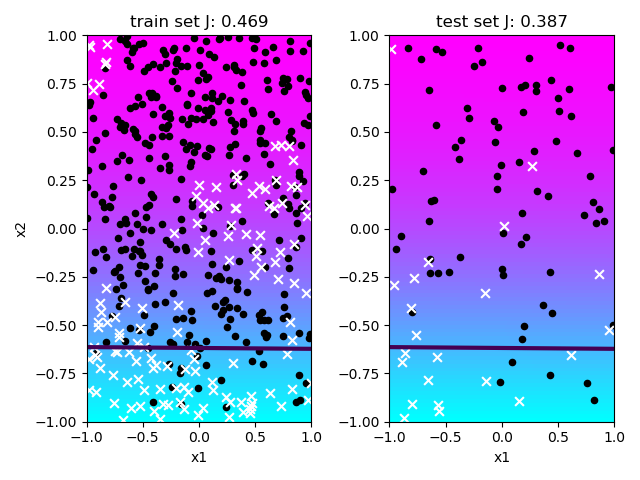
\includegraphics[scale=0.35]{plots/gradient_descent_1_1_2000.png}
				\captionsetup{justification=centering}
              \captionof{figure}{GD for 2000 Iterations \& Learning Rate of 1}
                \label{gradient_descent_1_1_2000}
\end{minipage}
    \textcolor{blue}{For 20 iterations the training error was 0.481 and the testing error was 0.418 in contrast the training \& testing error for 2000 iteration was 0.469 \& 0.387 respectively\\
With a smaller iteration we are getting a higher error rate while more iterations get a lower error rate, but with minimal difference.
The conclusion is that increasing the iteration, the error rate is optimized just by a minimum but more time consuming.
The iterations should be neither too low nor too high because if the iteration number is too high then although the result might be correct it just takes too long  to compute. On the other side they are too low the learning rate has not much time/chances to influence on the decision boundaries}

\item For degree $l = 2$ run GD for 200 iterations and learning rates of $\eta = .15$, $\eta = 1.5$ and $\eta = 15.$. Report training and test errors for each iteration number and plot the decision boundaries. Comment on the results and explain what is happening when $\eta$ is too large or too small.
\begin{minipage}[b]{0.4\textwidth}
  \vspace{10pt}
                  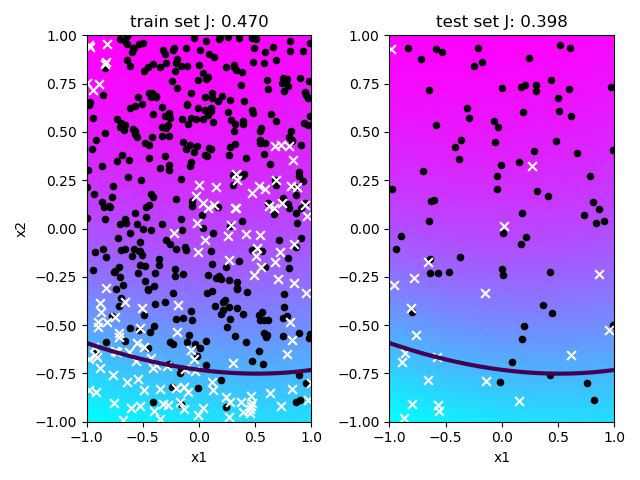
\includegraphics[scale=0.35]{plots/gradient_descent_2_0_15_200.png}
				 \captionsetup{justification=centering}
                  \captionof{figure}{GD for 200 Iterations \& Learning Rate of 0.15}
    \label{gradient_descent_2_0.15_200}
\end{minipage}
\hfill
\begin{minipage}[b]{0.4\textwidth}
            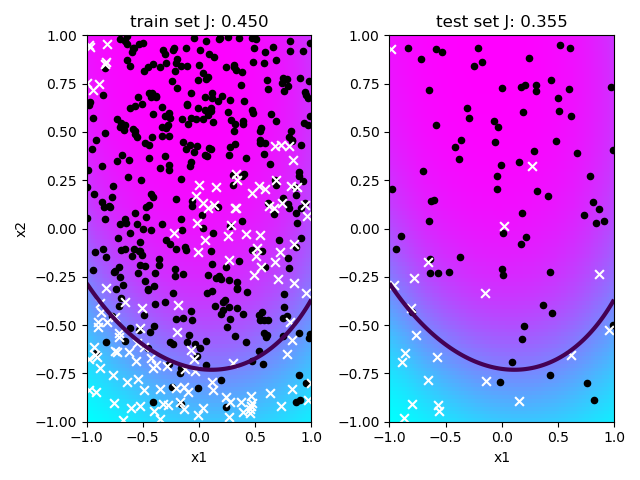
\includegraphics[scale=0.35]{plots/gradient_descent_2_1_5_200.png}
\captionsetup{justification=centering}
                  \captionof{figure}{GD for 200 Iterations \& Learning Rate of 1.5}
              \label{gradient_descent_2_1.5_200}
\end{minipage}
\begin{figure}[ht]
    \centering
  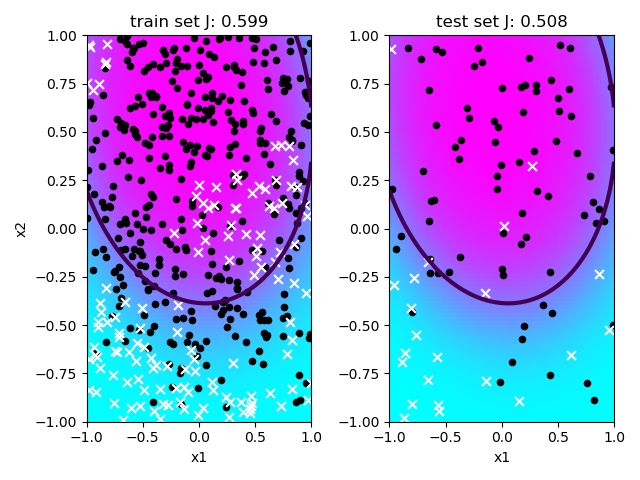
\includegraphics[scale=0.35]{plots/gradient_descent_2_15_200.png}
\captionsetup{justification=centering}
  \caption{GD for 200 Iterations \& Learning Rate of 15}
    \label{gradient_descent_2_15_200}
  \end{figure}

\noindent
\textcolor{blue}{For 200 iterations and a learning rate of 0.15 the training error was 0.470 and the testing error was 0.398. With a learning rate of 1.5 the training error was 0.450 and the testing error was 0.355. And with a learning rate of 15 the training error was 0.599 and the testing error was 0.508. \\
If the learning rate is too large the algorithm may overshoot the optimal point, so you end up at a non-optimal point with a higher error, on the other hand if it's to small than we have much more iterations to find the optimal point. Finding the optimal learning rate impacts directly the efficiency and reliability of the algorithm.}

\item Identify reasonably good pairs of values for the number of iterations and learning rate for each degree in $l \in {1, 2, 5, 15}$ that provides a good solution in reasonable time. Report these pairs, the performance obtained on training and testing set and plot each solution. Conclude by describing which degree seems the most appropriate to fit the given data.\\

\begin{minipage}[b]{0.4\textwidth}
  \vspace{10pt}
            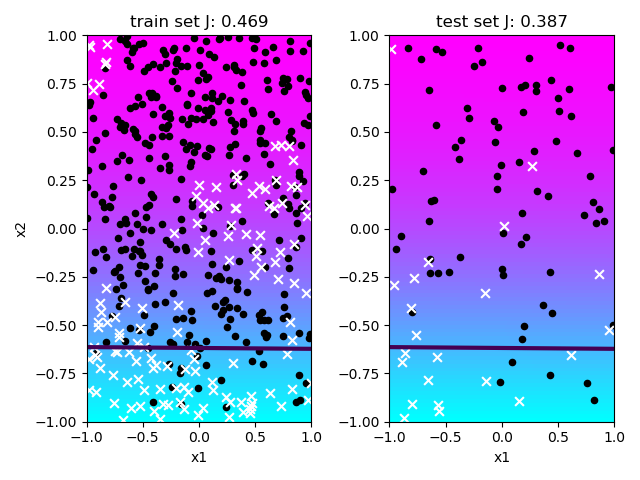
\includegraphics[scale=0.35]{plots/gradient_descent_1_2_250.png}
           \captionsetup{justification=centering}
            \captionof{figure}{Gradient Descend for degree 1, 250 iterations \& and a learning rate of 2}
  \label{gradient_descent_1_2_250}
\end{minipage}
\hfill
\begin{minipage}[b]{0.4\textwidth}
  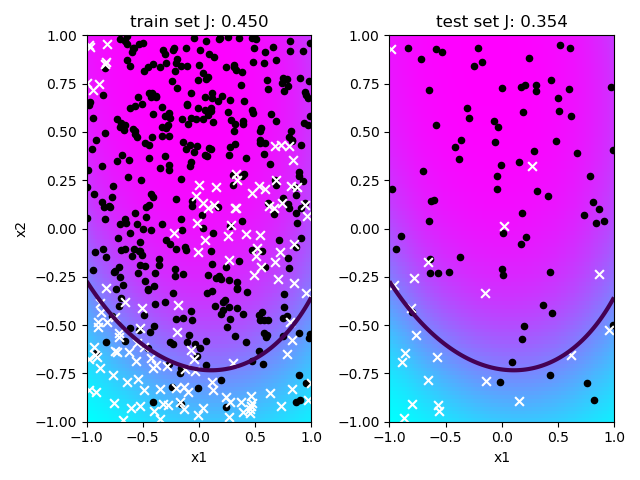
\includegraphics[scale=0.35]{plots/gradient_descent_2_2_250.png}
 \captionsetup{justification=centering}
  \captionof{figure}{Gradient Descend for degree 2, 250 iterations \& and a learning rate of 2}
  \label{gradient_descent_2_2_250}
\end{minipage}
\begin{minipage}[b]{0.4\textwidth}
  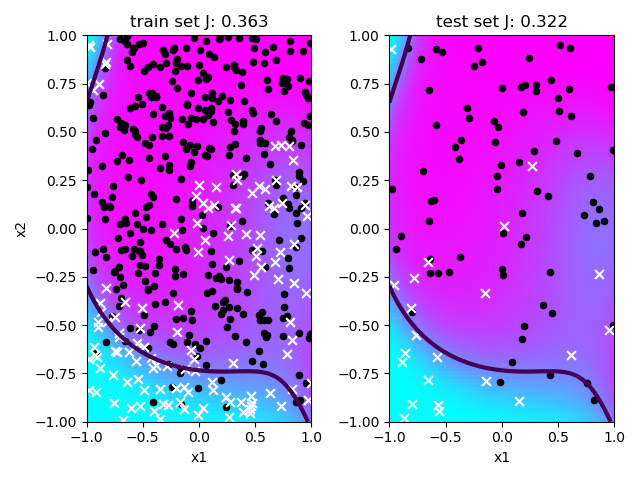
\includegraphics[scale=0.35]{plots/gradient_descent_5_2_250.png}
 \captionsetup{justification=centering}
  \captionof{figure}{Gradient Descend for degree 5, 250 iterations \& and a learning rate of 2}
  \label{gradient_descent_5_2_250}
\end{minipage}
\hfill
\begin{minipage}[b]{0.4\textwidth}
  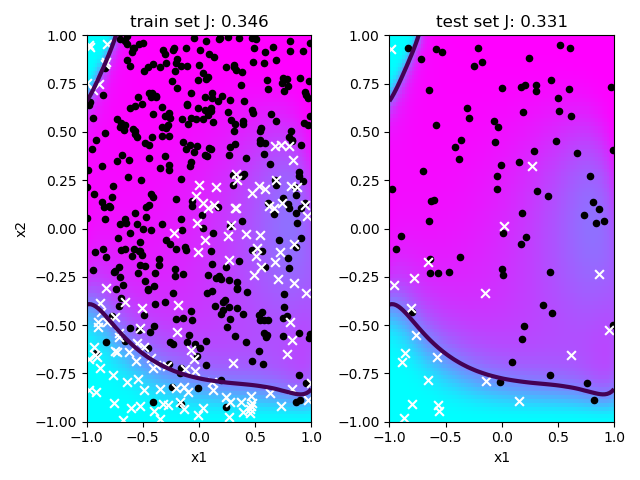
\includegraphics[scale=0.35]{plots/gradient_descent_15_2_250.png}
 \captionsetup{justification=centering}
  \captionof{figure}{Gradient Descend for degree 15, 250 iterations \& and a learning rate of 2}
  \label{gradient_descent_15_2_250}
\end{minipage}\\
\textcolor{blue}{By experimenting with different parameters we found out that a reasonably good pair of values for the number of iterations and learning rate for each degree in $l \in {1, 2, 5, 15}$ are 250 iterations \&  a learning rate of 2.
Using a fixed number of iteration and a fixed learning rate we got for degree 1 0.469 Trainings \& 0.387 Testing errors.   For degree 2 we got 0.450 Trainings \& 0.354 Testing errors. For degree 5 we got 0.363 Trainings \& 0.322 Testing errors. And for degree 15 we got 0.346 Trainings \& 0.331 Testing errors.  Due to a relatively low iteration number the computing was quite fast.      \\
With 250 iterations and a learning rate of 2, the degree 5 seems to be the most appropriate to fit the given data as we achieved with this degree the lowest testing error: 0.322.}
\item Describe a possible stopping criterium using the gradient of the cost function ?\\
\textcolor{blue}{A possible stopping criterium could be to stop as soon as the function gets close to zero or is equal zero.}
\end{enumerate}

\subsubsection{Adaptative gradient descent (GDad)}
\textbf{Fill the following blocks in the code you are provided:}
\begin{itemize}
\item In gradient\_descent.py implement the adaptive learning rate as follows: After every update check whether the cost increases or decreases.
\begin{compactenum}[-]
\item If the cost increased, reject the update (go back to the previous parameter setting) and multiply
the learning rate by 0.7.
\item If the cost decreased, accept the update and multiply the learning rate by 1.03.
\end{compactenum}
The iteration count should be increased after every iteration even if the update was rejected
\end{itemize}
\begin{enumerate}
\item Run GDad for varying degrees $l \in {1, 2, 5, 15}$ (with zero initialization of parameters, 1000 iterations, and initial learning rate $\eta = 1$). Report training and test errors, final learning rates and plot the hypothesis obtained in each case with function plot\_logreg in file logreg\_toolbox.py.\\
\begin{minipage}[b]{0.4\textwidth}
  \vspace{10pt}
  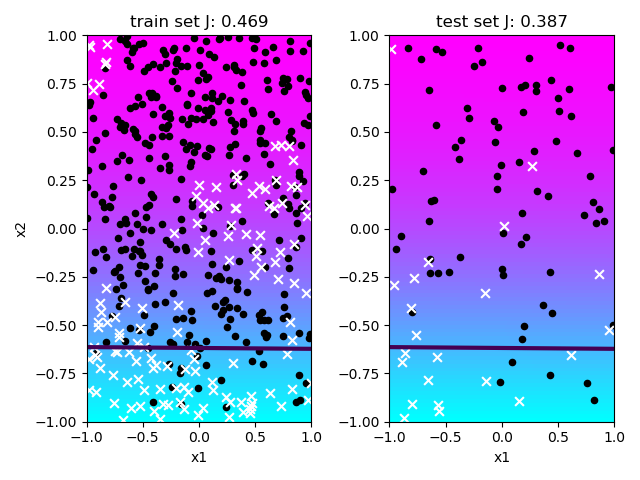
\includegraphics[scale=0.35]{plots/ad_gradient_descent_1_1_1000.png}
 \captionsetup{justification=centering}
  \captionof{figure}{Hypothesis for GDad for 1000 Iterations, a Learning Rate of 1 \& a Degree of 1}
  \label{ad_gradient_descent_1_1_1000}
\end{minipage}
\hfill
\begin{minipage}[b]{0.4\textwidth}
  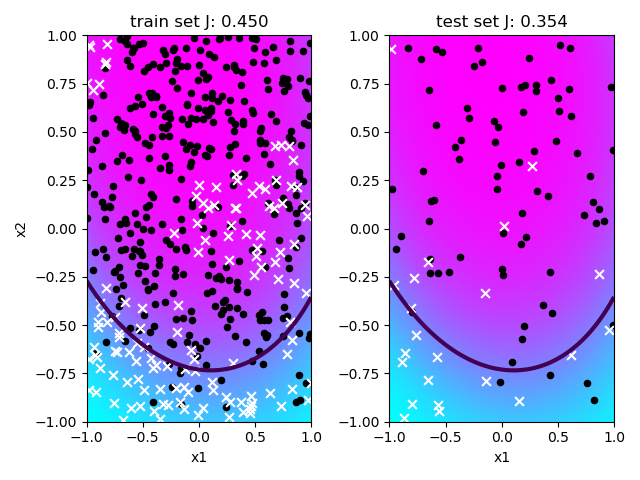
\includegraphics[scale=0.35]{plots/ad_gradient_descent_2_1_1000.png}
 \captionsetup{justification=centering}
  \captionof{figure}{Hypothesis for GDad for 1000 Iterations, a Learning Rate of 1 \& a Degree of 2}
  \label{ad_gradient_descent_2_1_1000}
\end{minipage}
\begin{minipage}[b]{0.4\textwidth}
  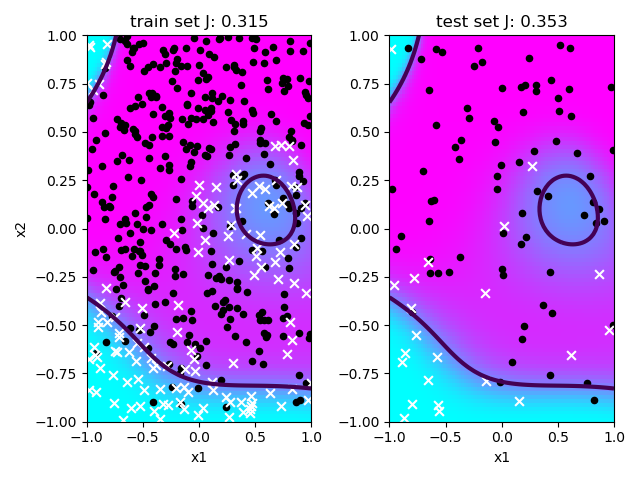
\includegraphics[scale=0.35]{plots/ad_gradient_descent_5_1_1000.png}
 \captionsetup{justification=centering}
  \captionof{figure}{Hypothesis for GDad for 1000 Iterations, a Learning Rate of 1 \& a Degree of 5}
  \label{ad_gradient_descent_5_1_1000}
\end{minipage}
\hfill
\begin{minipage}[b]{0.4\textwidth}
  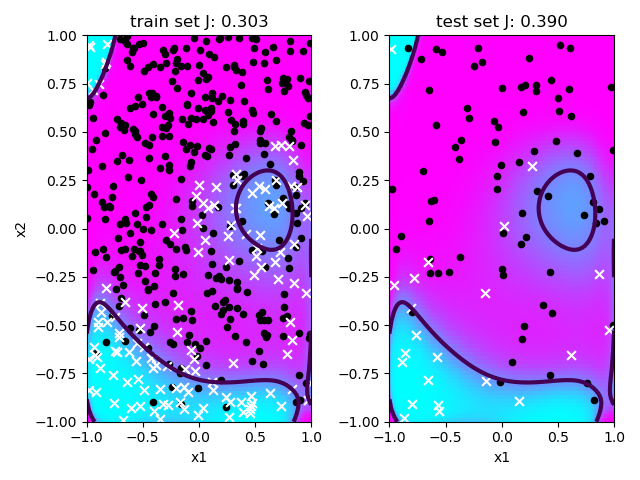
\includegraphics[scale=0.35]{plots/ad_gradient_descent_15_1_1000.png}
 \captionsetup{justification=centering}
  \captionof{figure}{Hypothesis for GDad for 1000 Iterations, a Learning Rate of 1 \& a Degree of 15}
  \label{ad_gradient_descent_15_1_1000}
\end{minipage}
\textcolor{blue}{With different degrees but constant iteration of 1000 and learning rate of 1 different testings \& trainings were computed as shown in the table below. }
\begin{table}[!h]
\centering
\label{GDad}
\begin{tabular}{|c|c|c|c|}
\hline
  \textbf{Degree} & \textbf{Training Error} & \textbf{Testing Error} & \textbf{Final Learning Rate} \\ \hline
  \textbf{1}      & 0.469                            & 0.387                  & 3.42e-09                              \\ \hline
  \textbf{2}      & 0.450                            & 0.354                  & 1.6e-08                               \\ \hline
  \textbf{5}      & 0.315                            & 0.353                  & 12.5                                  \\ \hline
  \textbf{15}     & 0.303                            & 0.390                  & 12.5                                  \\ \hline
\end{tabular}
\end{table}
\item  For each degree compare with the non-adaptive gradient descent variant. In particular, is the evolution of the learning rate numerically coherent with your previous guess of the optimal learning rate ? Discuss why GDad can be useful.\\
\begin{table}[!h]
\centering
\label{ad}
\begin{tabular}{|c|c|c|}
\hline
\textbf{Degree} & \textbf{Training Error} & \textbf{Testing Error} \\ \hline
\textbf{1}      & 0.469                  & 0.387                  \\ \hline
\textbf{2}      & 0.450                  & 0.354                  \\ \hline
\textbf{5}      & 0.349                  & 0.323                  \\ \hline
\textbf{15}     & 0.333                  & 0.342                  \\ \hline
\end{tabular}
\end{table}
\textcolor{blue}{If we compare the results for each degree of the adaptive gradient descent to the results of the non-adaptive
gradient descent it clearly shows that for low degrees for example a degree of 1 or 2 trainings \& testing errors are similar if not even the same. In Contrast for higher degrees like a degree of 5 or 15 the adaptive gradient descent performs better in terms of lower testing errors but it performs worse in terms of higher trainings errors. The evolution of the learning rate is not numerically coherent with our previous guess. \\
 GDad can be useful since it can often eliminates slow convergence and divergence issues. To do that the learning rate is decreased if the cost increased and increased if the cost decreased. }

\begin{minipage}[b]{0.4\textwidth}
  \vspace{10pt}
  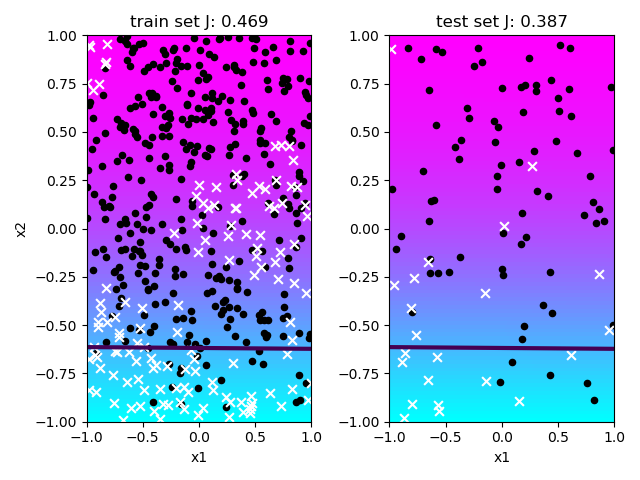
\includegraphics[scale=0.35]{plots/gradient_descent_1_1_1000.png}
 \captionsetup{justification=centering}
  \captionof{figure}{Hypothesis for GD for 1000 Iterations, a Learning Rate of 1 \& a Degree of 1}
  \label{gradient_descent_1_1_1000}
\end{minipage}
\hfill
\begin{minipage}[b]{0.4\textwidth}
  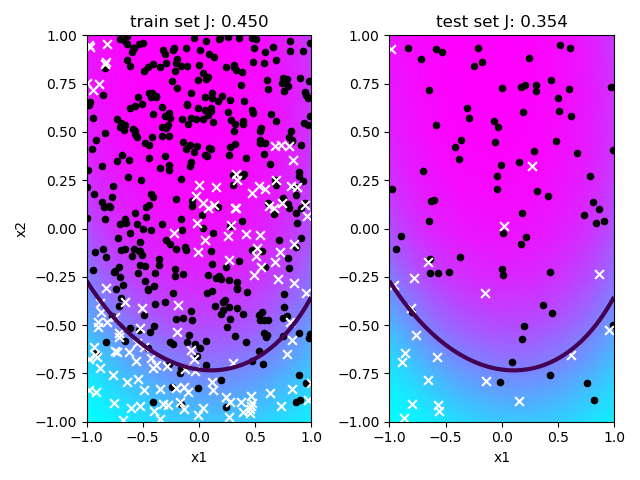
\includegraphics[scale=0.35]{plots/gradient_descent_2_1_1000.png}
 \captionsetup{justification=centering}
  \captionof{figure}{Hypothesis for GD for 1000 Iterations, a Learning Rate of 1 \& a Degree of 2}
  \label{gradient_descent_2_1_1000}
\end{minipage}
\begin{minipage}[b]{0.4\textwidth}
  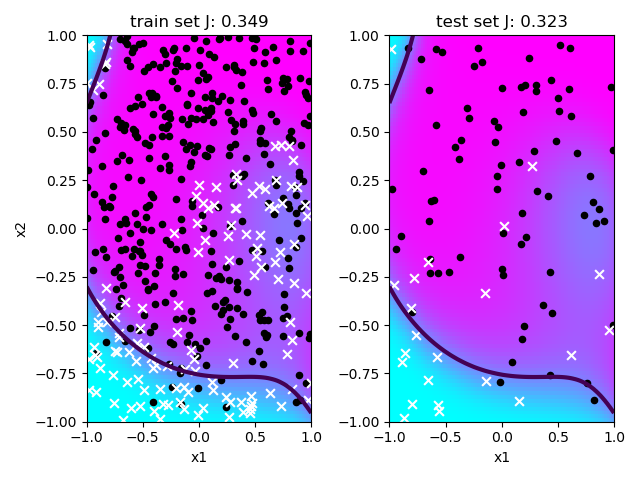
\includegraphics[scale=0.35]{plots/gradient_descent_5_1_1000.png}
 \captionsetup{justification=centering}
  \captionof{figure}{Hypothesis for GD for 1000 Iterations, a Learning Rate of 1 \& a Degree of 5}
  \label{gradient_descent_5_1_1000}
\end{minipage}
\hfill
\begin{minipage}[b]{0.4\textwidth}
  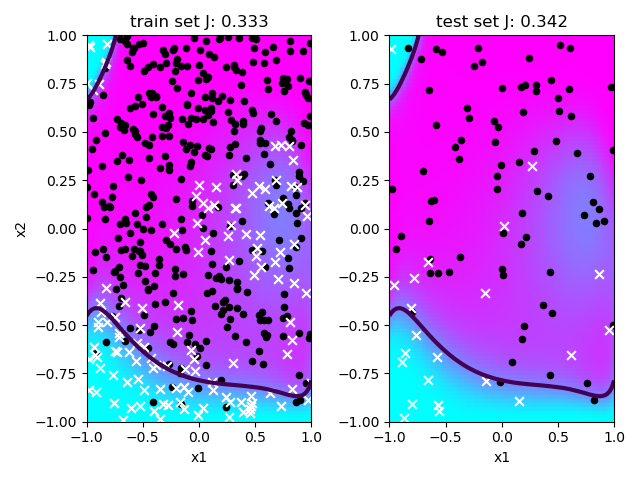
\includegraphics[scale=0.35]{plots/gradient_descent_15_1_1000.png}
 \captionsetup{justification=centering}
  \captionof{figure}{Hypothesis for GD for 1000 Iterations, a Learning Rate of 1 \& a Degree of 15}
  \label{gradient_descent_15_1_1000}
\end{minipage}

\end{enumerate}
\subsubsection{ Scipy optimizer}
In main\_logreg.py the VARIANT 3 is commented out. Un-comment the code and compare the results to the previous implementations.
\begin{enumerate}
\item Report training and test errors, and plot the hypothesis obtained for the four degrees $l \in {1, 2, 5, 15}$ with function plot\_logreg.\\

\begin{minipage}[b]{0.4\textwidth}
  \vspace{10pt}
  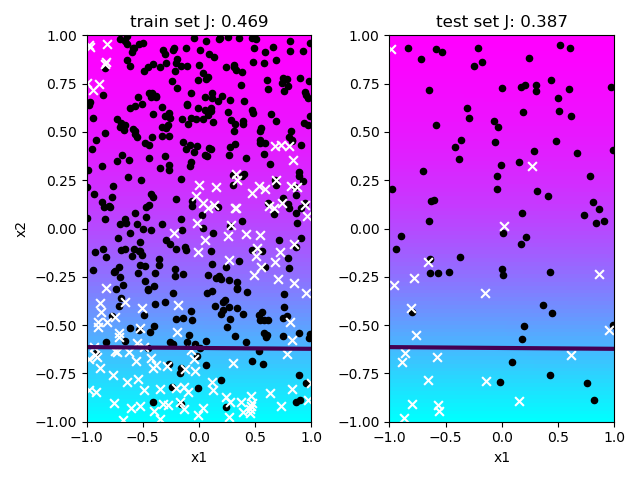
\includegraphics[scale=0.35]{plots/scipy_gradient_descent_1_1_1000.png}
 \captionsetup{justification=centering}
  \captionof{figure}{ Scipy Optimizer Plot for a Degree of 1}
  \label{scipy_gradient_descent_1_1_1000}
\end{minipage}
\hfill
\begin{minipage}[b]{0.4\textwidth}
  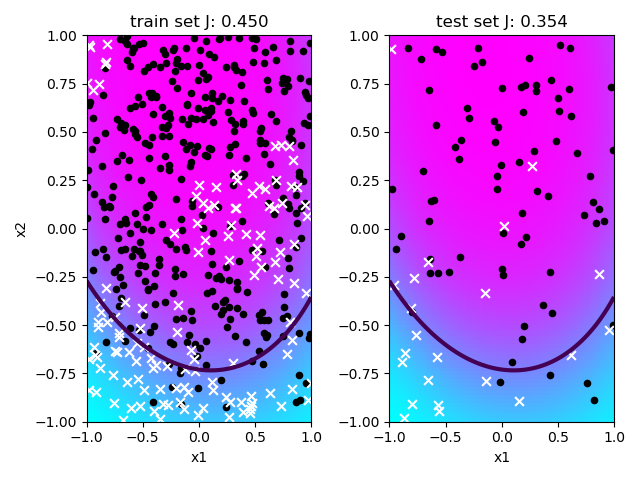
\includegraphics[scale=0.35]{plots/scipy_gradient_descent_2_1_1000.png}
 \captionsetup{justification=centering}
  \captionof{figure}{Scipy Optimizer Plot for a Degree of 2}
  \label{scipy_gradient_descent_2_1_1000}
\end{minipage}
\begin{minipage}[b]{0.4\textwidth}
  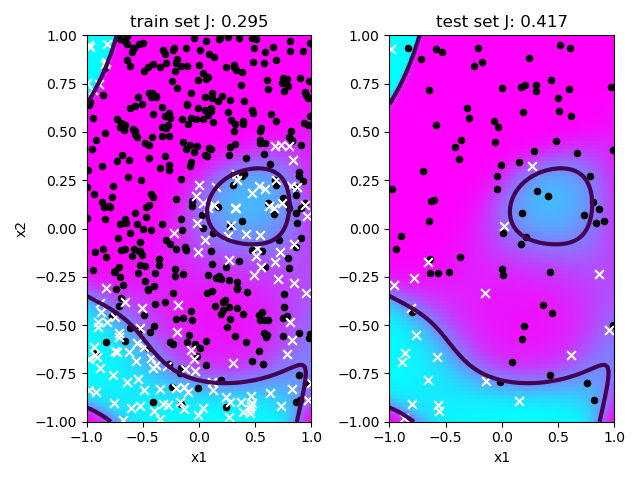
\includegraphics[scale=0.35]{plots/scipy_gradient_descent_5_1_1000.png}
 \captionsetup{justification=centering}
  \captionof{figure}{Scipy Optimizer Plot for a Degree of 5}
  \label{scipy_gradient_descent_5_1_1000}
\end{minipage}
\hfill
\begin{minipage}[b]{0.4\textwidth}
  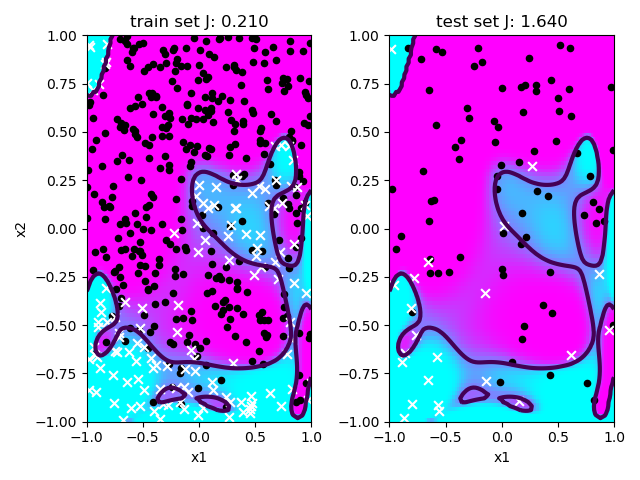
\includegraphics[scale=0.35]{plots/scipy_gradient_descent_15_1_1000.png}
 \captionsetup{justification=centering}
  \captionof{figure}{Scipy Optimizer Plot for a Degree of 15}
  \label{scipy_gradient_descent_15_1_1000}
\end{minipage}
\begin{table}[!h]
\centering
\caption{scipy}
\begin{tabular}{|c|c|c|}
\hline
\textbf{Degree} & \textbf{Trainings Error} & \textbf{Testing Error} \\ \hline
\textbf{1}      & 0.469                  & 0.387                  \\ \hline
\textbf{2}      & 0.450                  & 0.354                  \\ \hline
\textbf{5}      & 0.295                  & 0.417                  \\ \hline
\textbf{15}     & 0.210                  & 1.640                  \\ \hline
\end{tabular}
\end{table}
\item  Compare the results with those above (GD/GDad) and briefly discuss and interpret your observations. In particular does it change your opinion on which degree is best to fit the data?\\
\textcolor{blue}{The results for GD, GDad and Scipy optimizer are  for low degrees for example a degree of 1 or 2 for trainings \& testing errors similar if not even the same. In Contrast for higher degrees like a degree of 5 or 15 the scipy optimizer performs better in terms of lower trainings errors but it performs worse in terms of higher testing errors compared to  GD\&GDad.\\
It doesn't change our opinion on which degree is best to fit the data.}
\end{enumerate}

\end{document}